\documentclass[paper=a4, fontsize=11pt,twoside]{scrartcl}	
\usepackage[a4paper,pdftex]{geometry}	
\setlength{\oddsidemargin}{5mm}			
\setlength{\evensidemargin}{5mm}
\usepackage[protrusion=true,expansion=true]{microtype}	
\usepackage{amsmath,amsfonts,amsthm,amssymb}
\usepackage{graphicx}
\usepackage[spanish]{babel}
\usepackage[hidelinks]{hyperref}
\usepackage{hyperref}
\usepackage[hidelinks]{hyperref}
\usepackage{graphicx}
\usepackage{xcolor}
\usepackage{fancyhdr}
\newcommand{\HRule}[1]{\rule{\linewidth}{#1}} 	% Horizontal rule
\makeatletter							% Title
\def\printtitle{%						
    {\centering \@title\par}}
\makeatother									
\makeatletter							% Author
\def\printauthor{%					
    {\centering \large \@author}}				
\makeatother							
\title{	\normalsize \textsc{ANEXO DE DISEÑO DE SOFTWARE} 	% Subtitle
		 	\\[2.0cm]								% 2cm spacing
			\HRule{0.5pt} \\						% Upper rule
			\LARGE \textbf{\uppercase{Sistemas de posicionamiento de objetos mediante la tecnología Bluetooth Low Energy, modo Beacon}}	% Title
			\HRule{2pt} \\ [0.5cm]		% Lower rule + 0.5cm spacing
			\normalsize \today			% Todays date
		}
\author{
		Rubén Arce Domingo\\	
		Master en automatización y robótica\\	
		industrial\\
        \texttt{akimbo170@gmail.com} \\
}


\begin{document}
\thispagestyle{empty}		% Remove page numbering on this page
\printtitle					% Print the title data as defined above
  	\vfill
\printauthor				% Print the author data as defined above
\newpage
\cleardoublepage
\tableofcontents
\listoffigures
\cleardoublepage
\pagestyle{fancy}
\fancyfoot[R]{Rubén Arce}
\fancyfoot[L]{BLE Tracking - 2020}
\section{Introducción}
    Este proyecto engloba programación de 3 sistemas que emplean protocolos y tecnologías muy diferenciadas para llevar a cabo 
    la transmisión de información. Para lo cual se ha empleado el lenguaje de programación C para el firmware de los 
    microcontroladores y Python para llevar a cabo los cálculos de distancia y visualización de los beacons.
    \paragraph{}
    Se han llevado a cabo pruebas en interiores y exteriores, en una casa, en un supermercado y en un lugar con un número elevado de dispositivos BLE y
    a continuación se muestra el procedimiento y resultados.
\section{Firmware}
    \subsection{Emisor BLE o beacon}
        La ventaja de los beacons es que se ha llevado a cabo el paradigma de plug and play, es decir, tan solo hay que conectar la batería y comienza 
        a funcionar sin problemas. La única posibilidad de configuración podría ser el tiempo de envio de datos, teniendo en cuenta que estamos en fases 
        de pruebas no se ha adoptado un perfil demasiado conservador en lo que a batería se refiere. 

        En la versión real para cliente se le dará la posibilidad de configurar a su gusto la frecuencia de envio de datos con las conscuencias 
        que esto conlleva en la autonomía.
    \subsection{Receptor gateway o master}
        \subsubsection{Configuración inicial}
            El equipo que escucha a los beacons ha de hacer un barrido cada X tiempo, obtener el rssi y por último enviar a través de mqtt los datos 
            para que el sistema de visualización sea capaz de posicionarlos dentro de un mapa.
            Para que todo esto funciona es necesario que alguien les configure el Wifi al que han de conectarse para poder transmitir los datos,
            esta configuración inicial ha de ser sencilla y sobretodo ha de poderse cambiar en el caso de que la contraseña cambie o de que se desplacen 
            los equipos a otro lugar.
            
            Para ello se ha programado lo siguiente:
            \begin{enumerate}
                \item El Master intenta conectarse al wifi que tenga en memoria guardado, según sale de fábrica lo intenta con números aleatorios.
                \item Cuando fracase en el intento, generará un punto de acceso, es decir, se crea un wifi al que el usuario ha de conectarse.
                \item Una vez conectado a este wifi sin internet ha de meterse en la página web alojada en el 192.168.4.1 donde introducirá los credenciales 
                del wifi real al que ha de conectarse.
                \item Tras recibir los datos proporcionados por el cliente el equipo se conectará a internet y estará listo para usarse y escuchar beacons.
                \item Se guarda en memoria flash los datos para que cada vez que se apage no sea necesario repetir el proceso
            \end{enumerate}
            En todo momento si se quisiera volver a condiciones de fábrica se puede pulsar el botón a la vez que se enciende el dispositivo y se reseteará 
            la memoria previamente configurada y volverá a generarse el punto de acceso wifi para repetir el proceso.
            
            En la figura 1 se puede ver como es el interfaz web que se ha llevado a cabo para la configuración del wifi.
            \begin{center}
                \begin{figure}[]
                    \centering
                    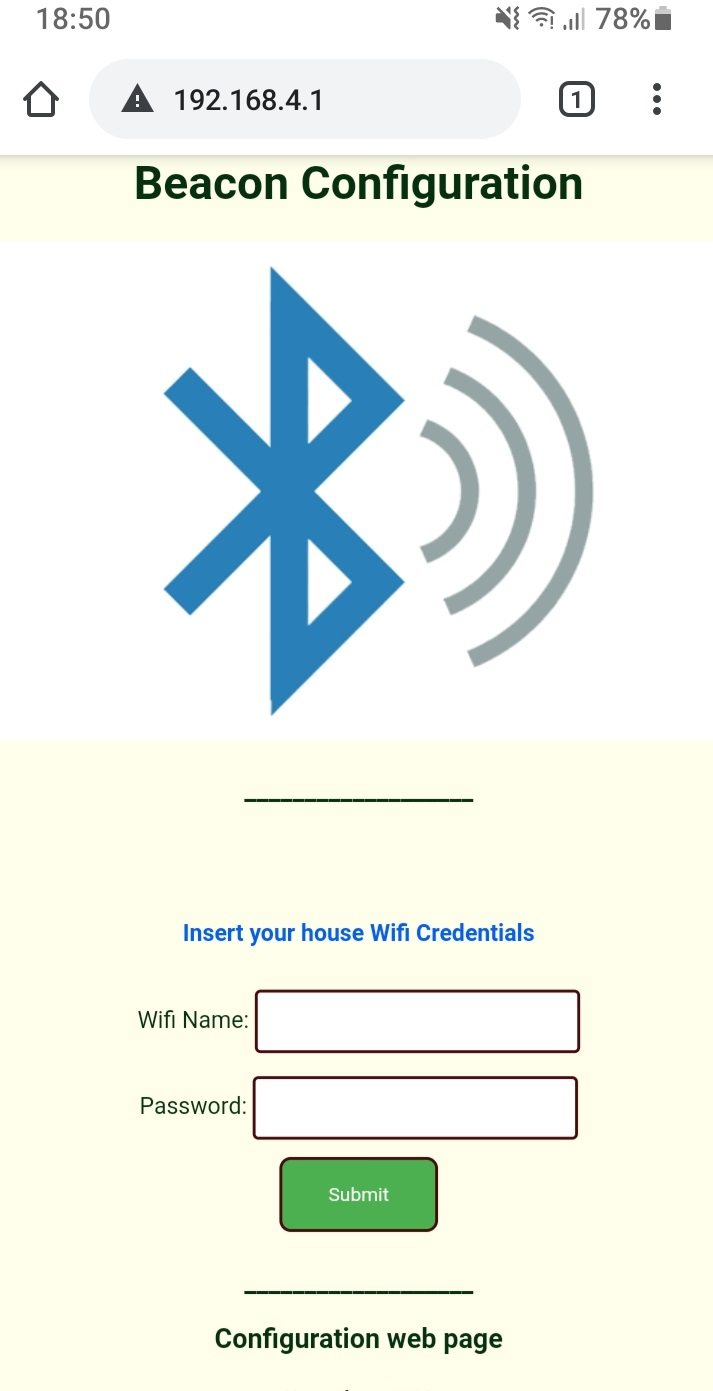
\includegraphics[width=0.3\textwidth]{../../Memmory/images/AP_wifi_config.jpeg}
                    \caption{Captura de pagina web generada por el dispositivo}
                    \label{fig:mesh12}
                \end{figure}
            \end{center}
        \subsubsection{Funcionamiento}
            Una vez llevada a cabo esta configuración inicial y conectados al terminal a través del puerto serie podemos ver como se lleva a cabo el barrido 
            de beacons y el procesamiento de los mismos.

            El envio de información a través de mqtt se lleva a cabo en el acto consiguiendo una frecuencia elevada de datos que alimentan a nuestra herramienta 
            de visualización de una forma dinámica. En la figura 2 se puede ver como en el primer barrido se encuentran 8 beacons y en el segundo solo 7.
            \begin{center}
                \begin{figure}[]
                    \centering
                    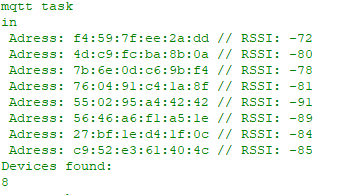
\includegraphics[width=0.5\textwidth]{../../Memmory/images/s_scanning_1.PNG}
                    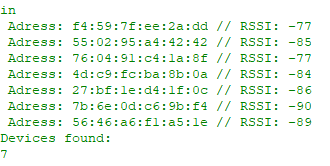
\includegraphics[width=0.5\textwidth]{../../Memmory/images/s_scanning_2.PNG}
                    \caption{Escaneo y procesamiento de dispositivos beacons}
                    \label{fig:mesh13}
                \end{figure}
            \end{center}
\section{Herramientas de visualización}
    \subsection{Tecnologías}
        Para generar las pantallas y animaciones he empleado Python con su librería "Pygame", en lo que respecta a los cálculos 
        y gráficas se ha empleado Matplotlib y para hacer operaciones de una forma rápida "NumPy".    
    \subsection{Procedimiento}
        Se han llevado a cabo 5 simulaciones, en todas ellas la metodología ha sido la siguiente:
        \begin{enumerate}
            \item Escucha de los datos
            \item Parseo de los mismos así como almacenamiento en estructuras de datos que permitan luego fácil utilización.
            \item Filtraje, cálculos de posicionamiento y ajustes.
            \item Visualización y escalado de los resultados.
        \end{enumerate}
    \subsection{Simulaciones}
        \subsubsection{Prueba de concepto}
            Para comprobar si la tecnología era capaz de llevar a cabo el posicionamiento de un equipo en un mapa de estableció un sencillo
            escenario en el que había tres equipos que escuchaban y 4 beacons. En la siguiente imagen se puede apreciar el sencillo escenario.

            En la imagen podemos ver los coloridos beacons próximos entre si y como si que es posible situarlos con relativa preción. En la imagen 
            vemos que los masters tienen los nombres A1, A2 y A3 respectivamente.
            \begin{center}
                \begin{figure}[]
                    \centering
                    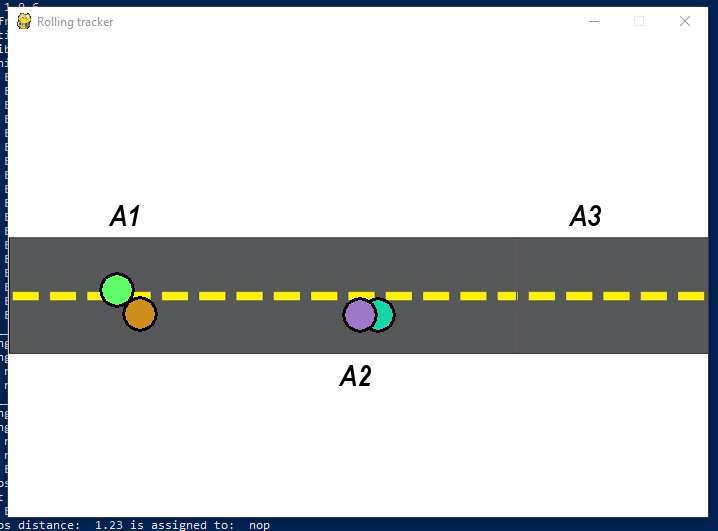
\includegraphics[width=0.7\textwidth]{../../Memmory/images/road_1.PNG}
                    \caption{Prueba piloto, carretera}
                    \label{fig:mesh14}
                \end{figure}
            \end{center}
        \subsubsection{Estabilidad del sistema}
            Tras esta primera prueba se optó por ver hasta que punto la tecnología es precisa, para lo cual se trazaron gráficas comparativas
            con los datos obtenidos a través de los equipos. En primer lugar se dejó durante un par de horas encendidos los equipos para ver las 
            fluctuaciones.

            Como podemos ver en la figura 4 las diferencias entre equipos estáticos son acusadas, es por ello por lo que queda demostrada la necesidad de
            desarrollar un filtro que anule este ruido radioeléctrico.
            \begin{center}
                \begin{figure}[]
                    \centering
                    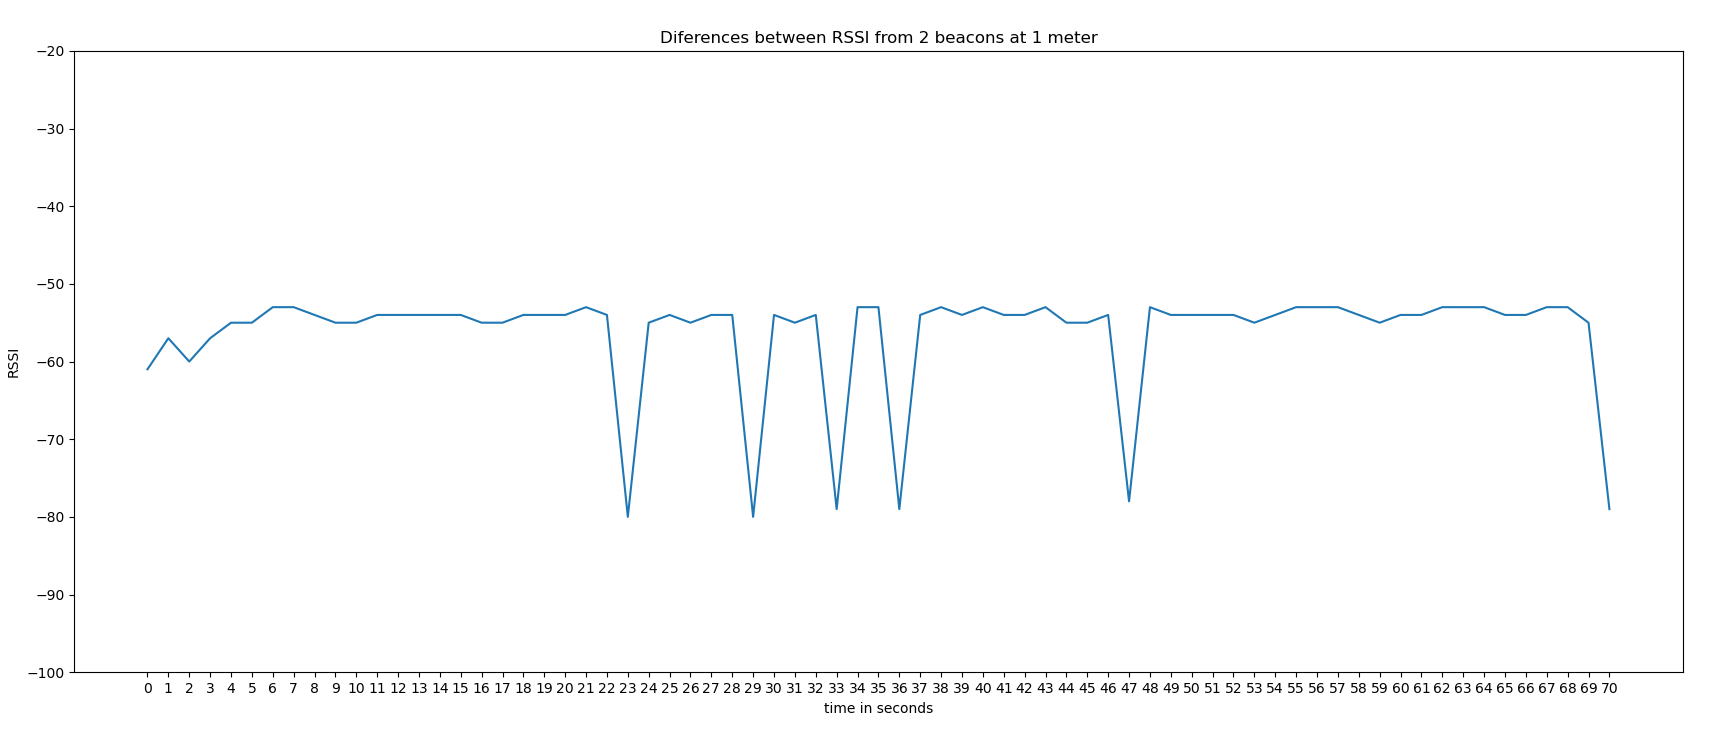
\includegraphics[width=1\textwidth]{../../Memmory/images/5min_beacon_rssi.PNG}
                    \caption{Toma de datos durante 2 horas}
                    \label{fig:mesh15}
                \end{figure}
            \end{center}
        \subsubsection{Posicionamiento real}
            El paso siguiente fue comprobar si tras filtrar las señales era realmente capaz de discernir si un Beacon se encontraba en una habitación
            o en otra tan solo atendiendo a su rssi, para lo cual se ha llevado a cabo una simulación que permite dibujar las dimensiones de las 
            habitaciones, la posición de los beacons e incluso el color de las mismas. En la figura 5 se puede ver una captura del archivo de configuración 
            con el que se pretende que caulquiera pueda dibujarse su propia casa.
            \begin{center}
                \begin{figure}[]
                    \centering
                    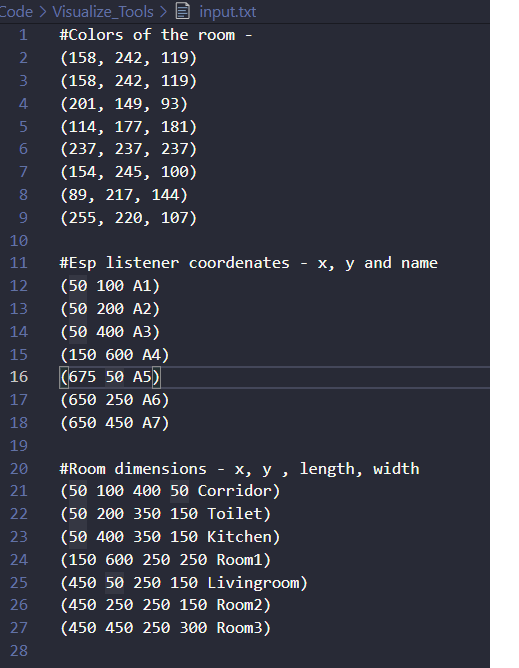
\includegraphics[width=0.5\textwidth]{../../Memmory/images/config_file_house.PNG}
                    \caption{Archivo de configuración de diseño de casa}
                    \label{fig:mesh16}
                \end{figure}
            \end{center}
            Una vez creada nuestra casa ya solo queda colocar realmente los equipos en lugares elevados y poco acesibles y ejecutar el script.
            Los equipos estuvieron durante una semana encendidos escuchando beacons y los resultados fueros los esperados. En la figura 6 se puede 
            visualizar el diseño de la casa en la que se llevó a cabo la prueba.
            \paragraph{}
            El caso más curioso de todos es que se dejaron beacons estáticos encima de armarios y la posición no móvil de los mismos 
            se mantuvo en la simulación en todo momento. En la imagen 7 se muestra como en todo momento fueron percibidos por los masters.
            \paragraph{}
            Al movernos dentro de la casa los masters de las habitaciones contiguas nos percibían con menor rssi, es por
            ello por lo que no nos visualizaba dentro de esa estancia. En la figura 8 se puede ver como los cuatro personas se 
            encontraban en el salón de la casa en ese momento.
            \begin{center}
                \begin{figure}[]
                    \centering
                    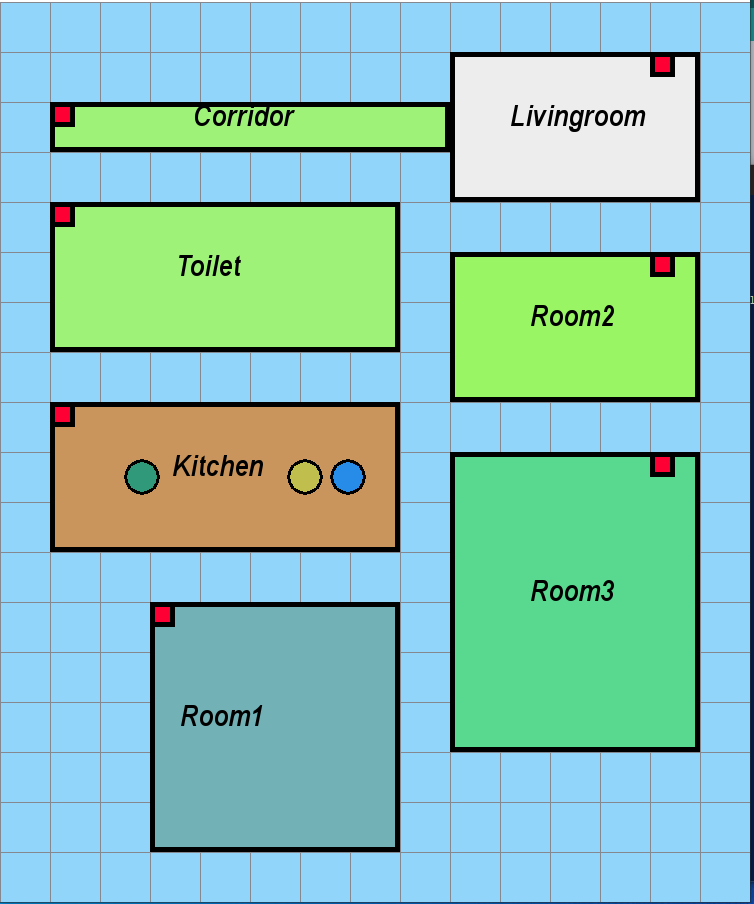
\includegraphics[width=0.5\textwidth]{../../Memmory/images/house_simulation_1.PNG}
                    \caption{Ejemplo de 3 personas dentro de una misma habitación}
                    \label{fig:mesh17}
                \end{figure}
            \end{center}          
            \begin{center}
                \begin{figure}[]
                    \centering
                    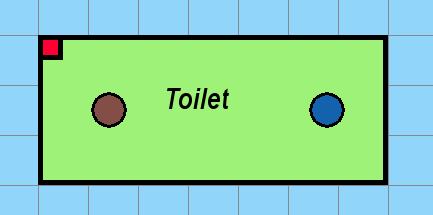
\includegraphics[width=0.5\textwidth]{../../Memmory/images/house_simulation_2.PNG}
                    \caption{Beacons estáticos durante la simulación}
                    \label{fig:mesh19}
                \end{figure}
            \end{center} 
            \begin{center}
                \begin{figure}[]
                    \centering
                    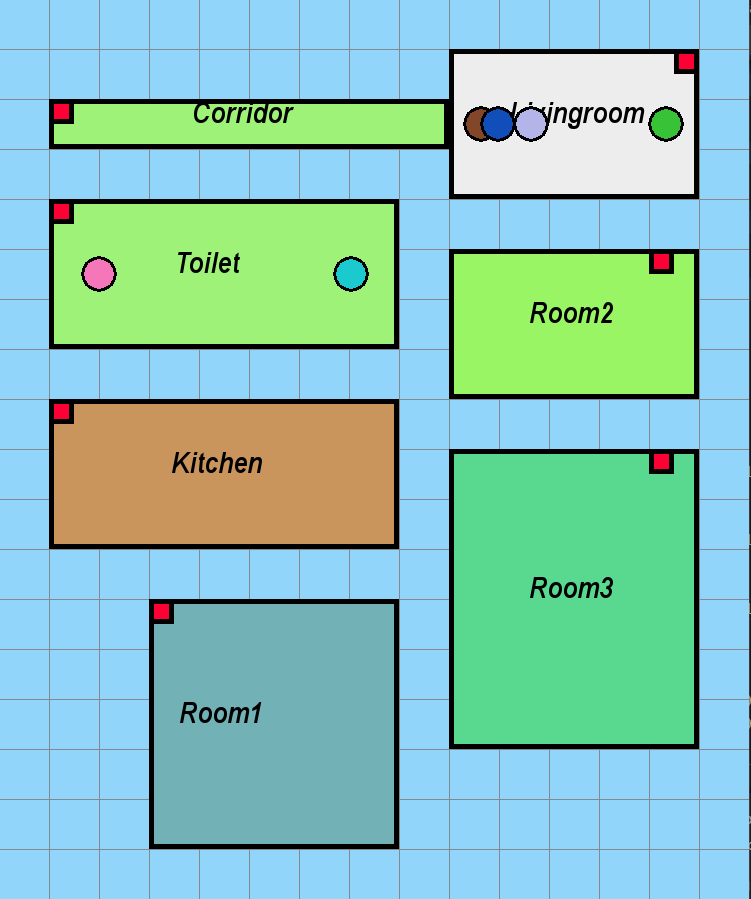
\includegraphics[width=0.5\textwidth]{../../Memmory/images/house_simulation_3.PNG}
                    \caption{Beacons en movimiento}
                    \label{fig:mesh18}
                \end{figure}
            \end{center}   
        \subsubsection{Prueba en supermercado}
            Una vez testada la tecnología se llevó a cabo una prueba real en un supermercado, para llevar a cabo el ejemplo
            se instalaron únicamente 2 masters y 6 beacons en carros en movimiento.
            Como suele pasar la prueba real no se parece tanto a las pruebas anteriores y podemos comprobar como 
            el algoritmo se complica más en asuncia de numerosos masters escuchando beacons, en este caso como solo se disponían
            de 2, los cálculos no siempre eran tan precisos y el filtro implementado en el caso de un desplazamiento rápido de un 
            equipo de punta a punta del supermercado no era el más óptimo.
            \begin{center}
                \begin{figure}[]
                    \centering
                    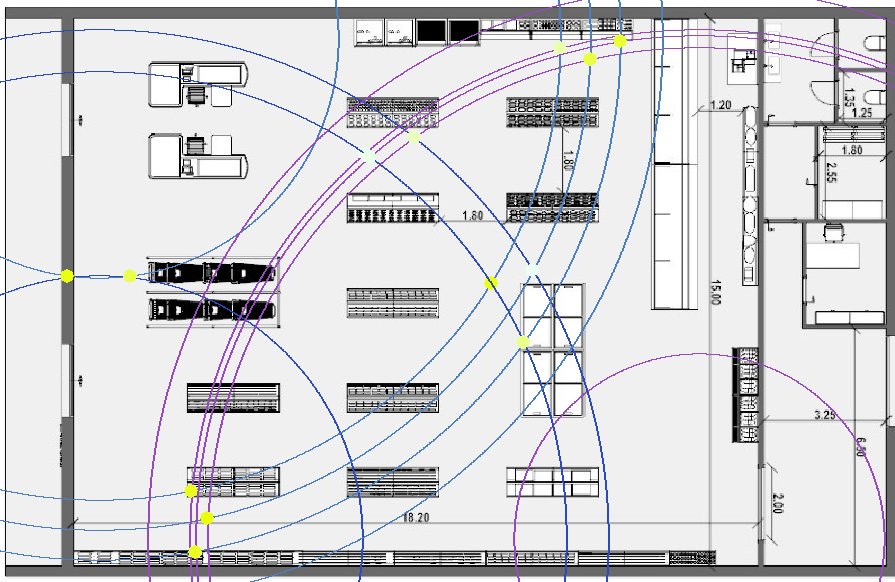
\includegraphics[width=0.7\textwidth]{../../Memmory/images/agrupation_3.PNG}
                    \caption{Beacons en movimiento dentro de supermercado captura 1}
                    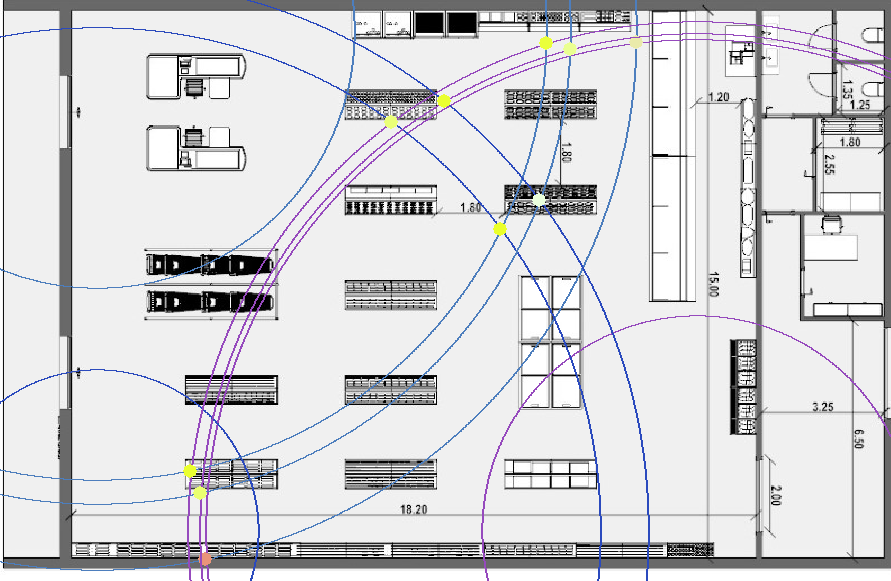
\includegraphics[width=0.7\textwidth]{../../Memmory/images/agrupation_2.PNG}
                    \caption{Beacons en movimiento dentro de supermercado captura 2}
                    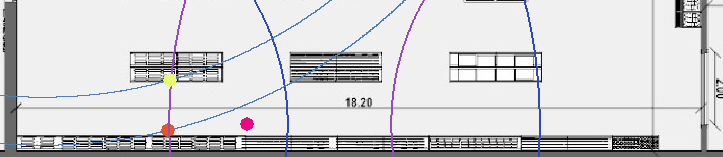
\includegraphics[width=0.5\textwidth]{../../Memmory/images/agrupation_1.PNG}
                    \caption{Beacons en supermercado percibidos solo por un master}
                    \label{fig:mesh10}
                \end{figure}
            \end{center}   
            
            Podemos ver como los puntos amarillos son los carros de la compra percibidos por ambos beacons y los rojos son aquellos
            que solo son escuchados por un master, de tal modo que el punto en el que se encuentran es menos preciso a menos número de 
            masters escuchando, igualmente se puede llevar a ver en que lugar hay más densidad de gente.

    \subsection{Conclusiones}
        Podemos concluir que la tecnología de posicionamiento de objetos o personas en interiores es suficientemente precisa como para 
        situar de una forma acertada dentro de una habitación.
        
        Se han de tener en cuenta de las limitaciones físicas que esto conlleva puesto
        que los equipos presentan fluctuaciones en su percepción de rssi así como de la influencia de medio en el que se coloquen.

        Aún con todo esto estamos ante un sistema perfectamente válido para la aplicación que tenemos entre manos siempre y cuando no se requiera de una
        exactitud o precisión elevada. 

        El mayor punto a favor de este sistema es su relación calidad precio, por escasos euros se puede colocar un dispositivos emisor y posicionarlo 
        sin miedo a que se pierda puesto que un sustituto sería asequible.

\end{document} 